\documentclass{article}

\usepackage[utf8]{inputenc}
\usepackage[english]{babel}
\usepackage{amsmath,amsfonts,amssymb}
\usepackage{fullpage}
\usepackage{verbatim}
\usepackage{xcolor}
\usepackage{subcaption}
\usepackage{float}
\usepackage{tikz,pgfplots}
\pgfplotsset{compat=1.18}

\pgfplotsset{
  width=150mm,height=100mm,
  major grid style={thin,dotted,color=black!50},
  minor grid style={thin,dotted,color=black!50},
  grid,
  every axis/.append style={
    line width=0.5pt,
    tick style={
      line cap=round,
      thin,
      major tick length=4pt,
      minor tick length=2pt,
    },
  },
  legend cell align=left,
  legend pos=north west,
  my colors/.style={
      cycle list={
          {blue, thin},
          {red, thin},
          {green!60!black, thin},
          {orange, thin},
          {purple, thin},
          {cyan!70!black, thin}
      }
  }
}

\begin{document}

\title{DeLI Benchmarks}
\author{}

\newcommand{\note}[1]{{\color{red}#1}}



%% IMPORT-DATA chisquared_data ../results_after_submission/benchmark_chisquared_uint32_20260429_212453.txt
%% IMPORT-DATA exponential_data ../results_after_submission/benchmark_exponential_uint32_20260429_073944.txt
%% IMPORT-DATA mix_gauss_data ../results_after_submission/benchmark_mix_gauss_uint32_20260429_140412.txt
%% IMPORT-DATA normal_data ../results_after_submission/benchmark_normal_uint32_20260429_011557.txt
%% IMPORT-DATA uniform_data ../results_after_submission/benchmark_uniform_uint32_20260428_185517.txt
%% IMPORT-DATA zipf_data ../results_after_submission/benchmark_zipf_uint32_20260430_035554.txt

% Merge everything in a single table, keeping the dataset name as a column:
%% SQL ALTER TABLE chisquared_data ADD COLUMN dataset_name TEXT DEFAULT 'chisquared';

%% SQL ALTER TABLE exponential_data ADD COLUMN dataset_name TEXT DEFAULT 'exponential';

%% SQL ALTER TABLE mix_gauss_data ADD COLUMN dataset_name TEXT DEFAULT 'mix_gauss';

%% SQL ALTER TABLE normal_data ADD COLUMN dataset_name TEXT DEFAULT 'normal';

%% SQL ALTER TABLE uniform_data ADD COLUMN dataset_name TEXT DEFAULT 'uniform';

%% SQL ALTER TABLE zipf_data ADD COLUMN dataset_name TEXT DEFAULT 'zipf';

%% SQL CREATE TABLE stats AS SELECT * FROM chisquared_data UNION ALL SELECT * FROM exponential_data UNION ALL SELECT * FROM mix_gauss_data UNION ALL SELECT * FROM normal_data UNION ALL SELECT * FROM uniform_data UNION ALL SELECT * FROM zipf_data;

%% SQL DELETE FROM stats WHERE index_name NOT LIKE '%DeLI%' OR workload_type == 'INSERT_DELETE';

%% SQL ALTER TABLE stats DROP COLUMN batch_no;

%% SQL ALTER TABLE stats DROP COLUMN batch_operations;

%% SQL ALTER TABLE stats DROP COLUMN conv_samples;

%% SQL ALTER TABLE stats DROP COLUMN conv_mean_throughput;

%% SQL ALTER TABLE stats DROP COLUMN conv_rse;

%% SQL ALTER TABLE stats DROP COLUMN adaptive_stop;

%% SQL CREATE TABLE stats_tmp AS SELECT index_name, index_variant, workload_type, init_num_keys, dataset_name, MEDIAN(total_time) AS total_time, MEDIAN(throughput) AS throughput FROM stats GROUP BY index_name, index_variant, workload_type, init_num_keys, dataset_name;

%% SQL DROP TABLE stats;

%% SQL ALTER TABLE stats_tmp RENAME TO stats;

%% SQL ALTER TABLE stats ADD COLUMN RHTOptimization TEXT;

%% SQL UPDATE stats SET RHTOptimization = substr(index_variant, 0, instr(index_variant, ';'));

%% SQL UPDATE stats SET index_variant = substr(index_variant, instr(index_variant, ';') + 1);

%% SQL ALTER TABLE stats ADD COLUMN SIMDLanes TEXT;

%% SQL UPDATE stats SET SIMDLanes = substr(index_variant, 0, instr(index_variant, ';'));

%% SQL UPDATE stats SET index_variant = substr(index_variant, instr(index_variant, ';') + 1);

%% SQL ALTER TABLE stats ADD COLUMN RHTLoad TEXT;

%% SQL UPDATE stats SET RHTLoad = substr(index_variant, 0, instr(index_variant, ';'));

%% SQL UPDATE stats SET index_variant = substr(index_variant, instr(index_variant, ';') + 1);

%% SQL ALTER TABLE stats ADD COLUMN TopOptimization TEXT;

%% SQL UPDATE stats SET TopOptimization = substr(index_variant, 0, instr(index_variant, ';'));

%% SQL UPDATE stats SET index_variant = substr(index_variant, instr(index_variant, ';') + 1);

%% SQL ALTER TABLE stats ADD COLUMN Highbits TEXT;

%% SQL UPDATE stats SET Highbits = substr(index_variant, 0, instr(index_variant, ';'));

%% SQL CREATE TABLE stats_best AS SELECT s.* FROM stats s JOIN (SELECT index_name, index_variant FROM (SELECT index_name, index_variant, ROW_NUMBER() OVER (PARTITION BY index_name ORDER BY SUM(total_time), index_variant) AS rn FROM stats GROUP BY index_name, index_variant) WHERE rn = 1) b ON s.index_name = b.index_name AND s.index_variant = b.index_variant;

%% SQL ALTER TABLE stats DROP COLUMN index_variant;


\section{DeLI Static Performance}\label{sec:deliconfig}

\subsection{Performance plot (all workloads and distributions)}

\begin{figure}[H]
\small
\centering

\begin{subfigure}{0.4\textwidth}
\centering
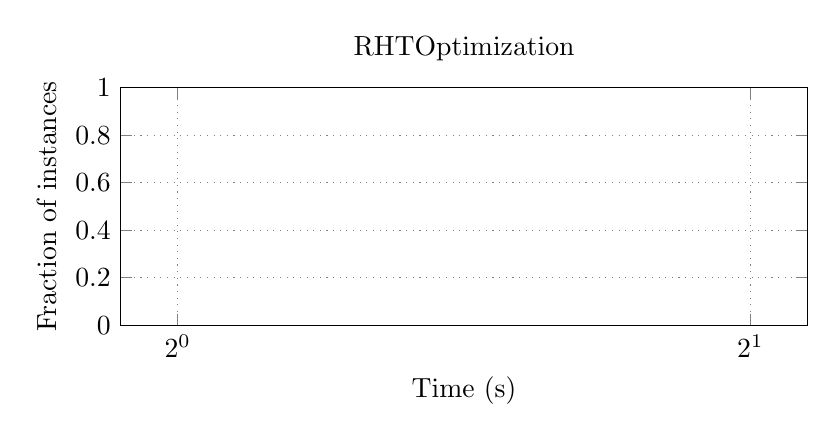
\begin{tikzpicture}
  \begin{axis}[
    my colors,
    title={RHTOptimization},
    xlabel={Time (s)},
    ylabel={Fraction of instances},
    xmode=log,
    log basis x={2},
    ymin=0.1,
    ymax=0.9,
    width=0.85\linewidth,
    height=4.6cm,
    grid=major,
    legend style={
        at={(1.02,0.5)},
        anchor=west,
        font=\small,
    },
    mark=*,
    mark size=0pt,
    line width=0.5pt
    ]
    %% MULTIPLOT \
    %% SELECT x, y, RHTOptimization as color FROM (
    %%   SELECT
    %%     total_time AS x,
    %%     (rn) * 1.0 / total_count AS y,
    %%     RHTOptimization,
    %%     ROW_NUMBER() OVER (PARTITION BY RHTOptimization, bucket ORDER BY total_time) as row_in_bucket
    %%   FROM (
    %%     SELECT
    %%       total_time,
    %%       RANK() OVER (PARTITION BY RHTOptimization ORDER BY total_time) as rn,
    %%       COUNT(*) OVER (PARTITION BY RHTOptimization) as total_count,
    %%       NTILE(500) OVER (PARTITION BY RHTOptimization ORDER BY total_time) AS bucket,
    %%       RHTOptimization
    %%     FROM stats
    %%     WHERE init_num_keys >= 1048576 AND index_name = 'DeLI-Static'
    %%   )
    %% )
    %% WHERE row_in_bucket = 1
    %% ORDER BY RHTOptimization, x
  \end{axis}
\end{tikzpicture}
\end{subfigure}
\newline

\begin{subfigure}{0.4\textwidth}
\centering
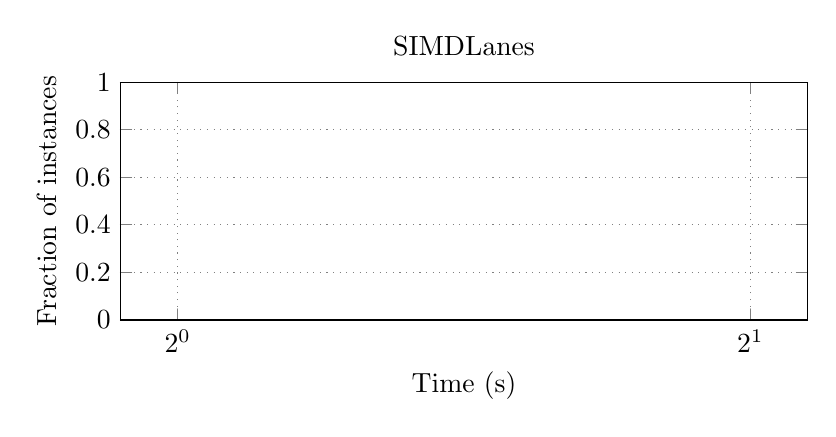
\begin{tikzpicture}
  \begin{axis}[
    my colors,
    title={SIMDLanes},
    xlabel={Time (s)},
    ylabel={Fraction of instances},
    xmode=log,
    log basis x={2},
    ymin=0.1,
    ymax=0.9,
    width=0.85\linewidth,
    height=4.6cm,
    grid=major,
    legend style={
        at={(1.02,0.5)},
        anchor=west,
        font=\small,
    },
    mark=*,
    mark size=0pt,
    line width=0.5pt
    ]
    %% MULTIPLOT \
    %% SELECT x, y, SIMDLanes as color FROM (
    %%   SELECT
    %%     total_time AS x,
    %%     (rn) * 1.0 / total_count AS y,
    %%     SIMDLanes,
    %%     ROW_NUMBER() OVER (PARTITION BY SIMDLanes, bucket ORDER BY total_time) as row_in_bucket
    %%   FROM (
    %%     SELECT
    %%       total_time,
    %%       RANK() OVER (PARTITION BY SIMDLanes ORDER BY total_time) as rn,
    %%       COUNT(*) OVER (PARTITION BY SIMDLanes) as total_count,
    %%       NTILE(500) OVER (PARTITION BY SIMDLanes ORDER BY total_time) AS bucket,
    %%       SIMDLanes
    %%     FROM stats
    %%     WHERE init_num_keys >= 1048576 AND index_name = 'DeLI-Static'
    %%   )
    %% )
    %% WHERE row_in_bucket = 1
    %% ORDER BY SIMDLanes, x
  \end{axis}
\end{tikzpicture}
\end{subfigure}
\newline

\begin{subfigure}{0.4\textwidth}
\centering
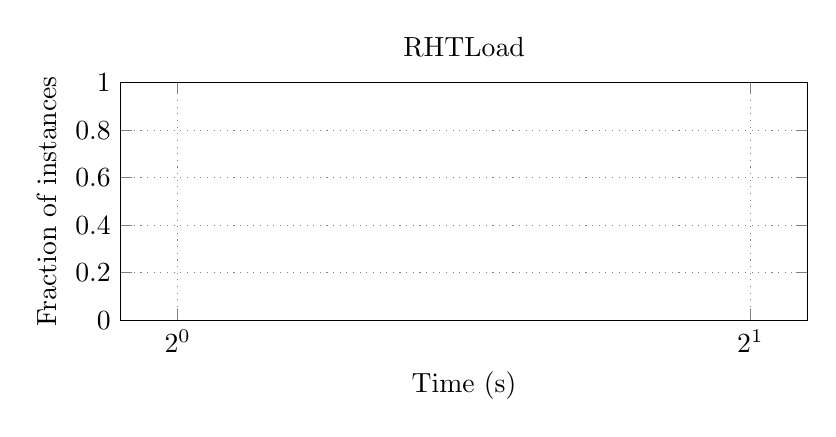
\begin{tikzpicture}
  \begin{axis}[
    my colors,
    title={RHTLoad},
    xlabel={Time (s)},
    ylabel={Fraction of instances},
    xmode=log,
    log basis x={2},
    ymin=0.1,
    ymax=0.9,
    width=0.85\linewidth,
    height=4.6cm,
    grid=major,
    legend style={
        at={(1.02,0.5)},
        anchor=west,
        font=\small,
    },
    mark=*,
    mark size=0pt,
    line width=0.5pt
    ]
    %% MULTIPLOT \
    %% SELECT x, y, RHTLoad as color FROM (
    %%   SELECT
    %%     total_time AS x,
    %%     (rn) * 1.0 / total_count AS y,
    %%     RHTLoad,
    %%     ROW_NUMBER() OVER (PARTITION BY RHTLoad, bucket ORDER BY total_time) as row_in_bucket
    %%   FROM (
    %%     SELECT
    %%       total_time,
    %%       RANK() OVER (PARTITION BY RHTLoad ORDER BY total_time) as rn,
    %%       COUNT(*) OVER (PARTITION BY RHTLoad) as total_count,
    %%       NTILE(500) OVER (PARTITION BY RHTLoad ORDER BY total_time) AS bucket,
    %%       RHTLoad
    %%     FROM stats
    %%     WHERE init_num_keys >= 1048576 AND index_name = 'DeLI-Static'
    %%   )
    %% )
    %% WHERE row_in_bucket = 1
    %% ORDER BY RHTLoad, x
  \end{axis}
\end{tikzpicture}
\end{subfigure}
\newline

\begin{subfigure}{0.4\textwidth}
\centering
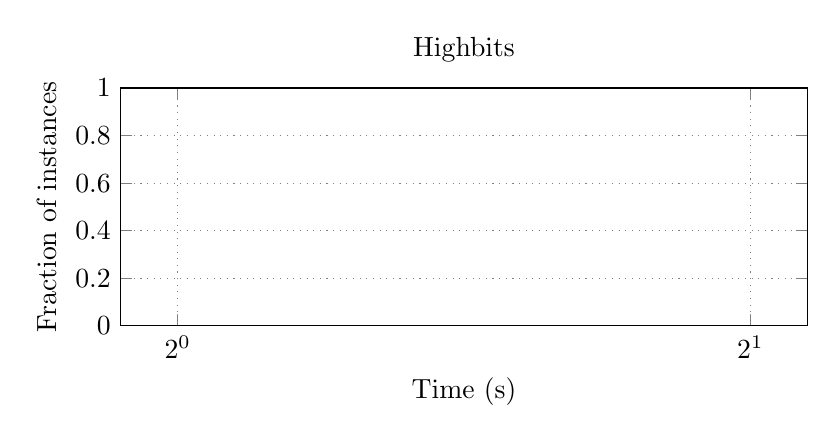
\begin{tikzpicture}
  \begin{axis}[
    my colors,
    title={Highbits},
    xlabel={Time (s)},
    ylabel={Fraction of instances},
    xmode=log,
    log basis x={2},
    ymin=0.1,
    ymax=0.9,
    width=0.85\linewidth,
    height=4.6cm,
    grid=major,
    legend style={
        at={(1.02,0.5)},
        anchor=west,
        font=\small,
    },
    mark=*,
    mark size=0pt,
    line width=0.5pt
    ]
    %% MULTIPLOT \
    %% SELECT x, y, Highbits as color FROM (
    %%   SELECT
    %%     total_time AS x,
    %%     (rn) * 1.0 / total_count AS y,
    %%     Highbits,
    %%     ROW_NUMBER() OVER (PARTITION BY Highbits, bucket ORDER BY total_time) as row_in_bucket
    %%   FROM (
    %%     SELECT
    %%       total_time,
    %%       RANK() OVER (PARTITION BY Highbits ORDER BY total_time) as rn,
    %%       COUNT(*) OVER (PARTITION BY Highbits) as total_count,
    %%       NTILE(500) OVER (PARTITION BY Highbits ORDER BY total_time) AS bucket,
    %%       Highbits
    %%     FROM stats
    %%     WHERE init_num_keys >= 1048576 AND index_name = 'DeLI-Static'
    %%   )
    %% )
    %% WHERE row_in_bucket = 1
    %% ORDER BY Highbits, x
  \end{axis}
\end{tikzpicture}
\end{subfigure}
\newline

\caption{Performance plots for DeLI-Static index on all workloads and distributions (init key size $2^{i}, i \in [20 , 25]$).}
\end{figure}



\section{DeLI Dynamic}\label{sec:deliconfig}

\subsection{Performance plot (all workloads and distributions)}

\begin{figure}[H]
\small
\centering

\begin{subfigure}{0.4\textwidth}
\centering
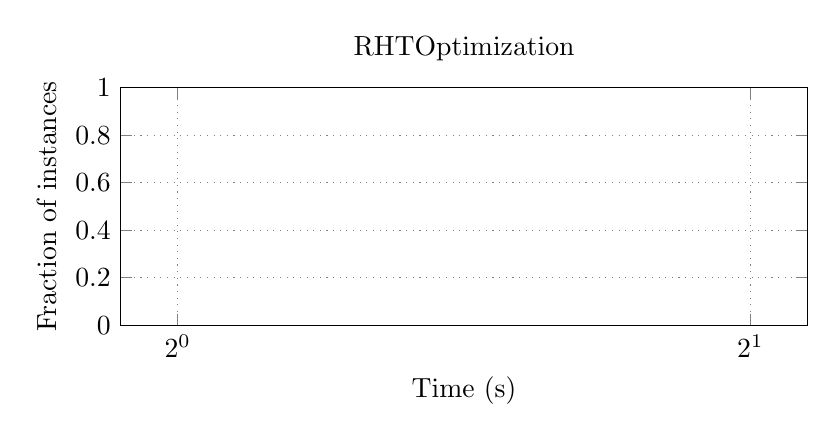
\begin{tikzpicture}
  \begin{axis}[
    my colors,
    title={RHTOptimization},
    xlabel={Time (s)},
    ylabel={Fraction of instances},
    xmode=log,
    log basis x={2},
    ymin=0.1,
    ymax=0.9,
    width=0.85\linewidth,
    height=4.6cm,
    grid=major,
    legend style={
        at={(1.02,0.5)},
        anchor=west,
        font=\small,
    },
    mark=*,
    mark size=0pt,
    line width=0.5pt
    ]
    %% MULTIPLOT \
    %% SELECT x, y, RHTOptimization as color FROM (
    %%   SELECT
    %%     total_time AS x,
    %%     (rn) * 1.0 / total_count AS y,
    %%     RHTOptimization,
    %%     ROW_NUMBER() OVER (PARTITION BY RHTOptimization, bucket ORDER BY total_time) as row_in_bucket
    %%   FROM (
    %%     SELECT
    %%       total_time,
    %%       RANK() OVER (PARTITION BY RHTOptimization ORDER BY total_time) as rn,
    %%       COUNT(*) OVER (PARTITION BY RHTOptimization) as total_count,
    %%       NTILE(500) OVER (PARTITION BY RHTOptimization ORDER BY total_time) AS bucket,
    %%       RHTOptimization
    %%     FROM stats
    %%     WHERE init_num_keys >= 1048576 AND index_name = 'DeLI-Dynamic'
    %%   )
    %% )
    %% WHERE row_in_bucket = 1
    %% ORDER BY RHTOptimization, x
  \end{axis}
\end{tikzpicture}
\end{subfigure}
\newline

\begin{subfigure}{0.4\textwidth}
\centering
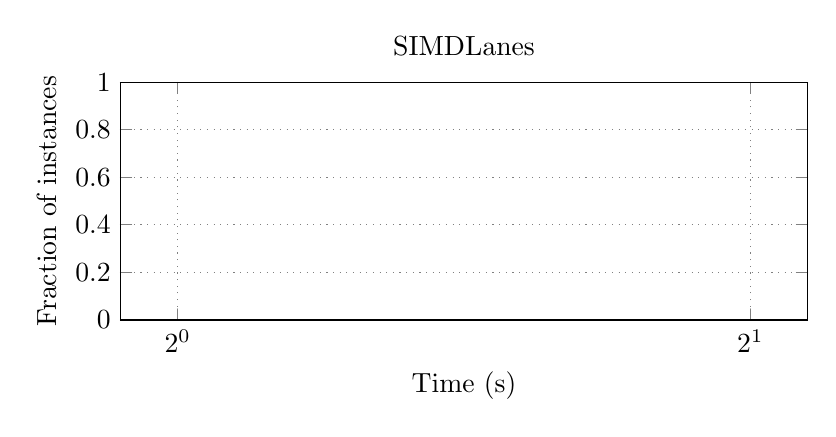
\begin{tikzpicture}
  \begin{axis}[
    my colors,
    title={SIMDLanes},
    xlabel={Time (s)},
    ylabel={Fraction of instances},
    xmode=log,
    log basis x={2},
    ymin=0.1,
    ymax=0.9,
    width=0.85\linewidth,
    height=4.6cm,
    grid=major,
    legend style={
        at={(1.02,0.5)},
        anchor=west,
        font=\small,
    },
    mark=*,
    mark size=0pt,
    line width=0.5pt
    ]
    %% MULTIPLOT \
    %% SELECT x, y, SIMDLanes as color FROM (
    %%   SELECT
    %%     total_time AS x,
    %%     (rn) * 1.0 / total_count AS y,
    %%     SIMDLanes,
    %%     ROW_NUMBER() OVER (PARTITION BY SIMDLanes, bucket ORDER BY total_time) as row_in_bucket
    %%   FROM (
    %%     SELECT
    %%       total_time,
    %%       RANK() OVER (PARTITION BY SIMDLanes ORDER BY total_time) as rn,
    %%       COUNT(*) OVER (PARTITION BY SIMDLanes) as total_count,
    %%       NTILE(500) OVER (PARTITION BY SIMDLanes ORDER BY total_time) AS bucket,
    %%       SIMDLanes
    %%     FROM stats
    %%     WHERE init_num_keys >= 1048576 AND index_name = 'DeLI-Dynamic'
    %%   )
    %% )
    %% WHERE row_in_bucket = 1
    %% ORDER BY SIMDLanes, x
  \end{axis}
\end{tikzpicture}
\end{subfigure}
\newline

\begin{subfigure}{0.4\textwidth}
\centering
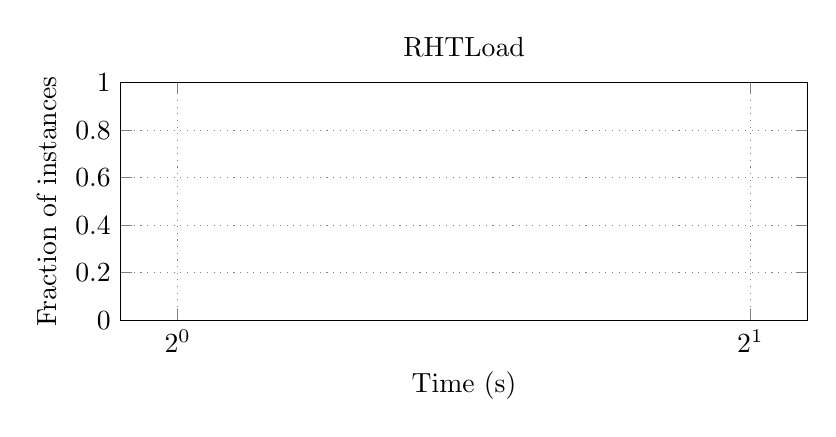
\begin{tikzpicture}
  \begin{axis}[
    my colors,
    title={RHTLoad},
    xlabel={Time (s)},
    ylabel={Fraction of instances},
    xmode=log,
    log basis x={2},
    ymin=0.1,
    ymax=0.9,
    width=0.85\linewidth,
    height=4.6cm,
    grid=major,
    legend style={
        at={(1.02,0.5)},
        anchor=west,
        font=\small,
    },
    mark=*,
    mark size=0pt,
    line width=0.5pt
    ]
    %% MULTIPLOT \
    %% SELECT x, y, RHTLoad as color FROM (
    %%   SELECT
    %%     total_time AS x,
    %%     (rn) * 1.0 / total_count AS y,
    %%     RHTLoad,
    %%     ROW_NUMBER() OVER (PARTITION BY RHTLoad, bucket ORDER BY total_time) as row_in_bucket
    %%   FROM (
    %%     SELECT
    %%       total_time,
    %%       RANK() OVER (PARTITION BY RHTLoad ORDER BY total_time) as rn,
    %%       COUNT(*) OVER (PARTITION BY RHTLoad) as total_count,
    %%       NTILE(500) OVER (PARTITION BY RHTLoad ORDER BY total_time) AS bucket,
    %%       RHTLoad
    %%     FROM stats
    %%     WHERE init_num_keys >= 1048576 AND index_name = 'DeLI-Dynamic'
    %%   )
    %% )
    %% WHERE row_in_bucket = 1
    %% ORDER BY RHTLoad, x
  \end{axis}
\end{tikzpicture}
\end{subfigure}
\newline

\begin{subfigure}{0.4\textwidth}
\centering
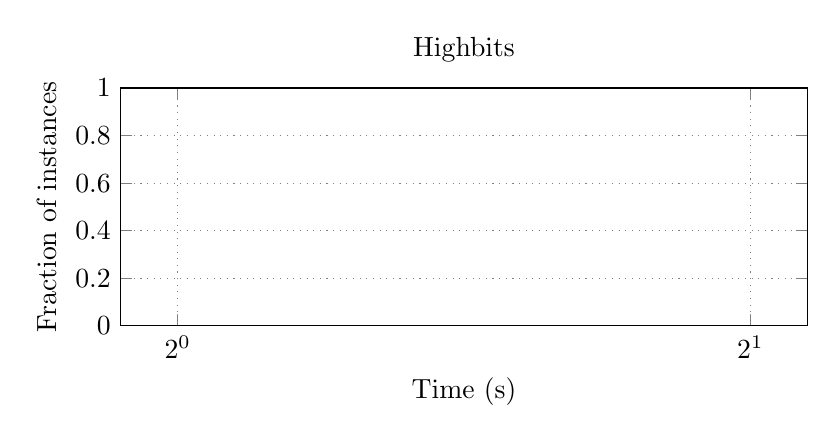
\begin{tikzpicture}
  \begin{axis}[
    my colors,
    title={Highbits},
    xlabel={Time (s)},
    ylabel={Fraction of instances},
    xmode=log,
    log basis x={2},
    ymin=0.1,
    ymax=0.9,
    width=0.85\linewidth,
    height=4.6cm,
    grid=major,
    legend style={
        at={(1.02,0.5)},
        anchor=west,
        font=\small,
    },
    mark=*,
    mark size=0pt,
    line width=0.5pt
    ]
    %% MULTIPLOT \
    %% SELECT x, y, Highbits as color FROM (
    %%   SELECT
    %%     total_time AS x,
    %%     (rn) * 1.0 / total_count AS y,
    %%     Highbits,
    %%     ROW_NUMBER() OVER (PARTITION BY Highbits, bucket ORDER BY total_time) as row_in_bucket
    %%   FROM (
    %%     SELECT
    %%       total_time,
    %%       RANK() OVER (PARTITION BY Highbits ORDER BY total_time) as rn,
    %%       COUNT(*) OVER (PARTITION BY Highbits) as total_count,
    %%       NTILE(500) OVER (PARTITION BY Highbits ORDER BY total_time) AS bucket,
    %%       Highbits
    %%     FROM stats
    %%     WHERE init_num_keys >= 1048576 AND index_name = 'DeLI-Dynamic'
    %%   )
    %% )
    %% WHERE row_in_bucket = 1
    %% ORDER BY Highbits, x
  \end{axis}
\end{tikzpicture}
\end{subfigure}
\newline

\caption{Performance plots for DeLI-Dynamic index on all workloads and distributions (init key size $2^{i}, i \in [20 , 25]$).}
\end{figure}

\section{DeLI Static Payload}\label{sec:delistaticpayload}

\subsection{Performance plot (all workloads and distributions)}

\begin{figure}[H]
\small
\centering

\begin{subfigure}{0.24\textwidth}
\centering
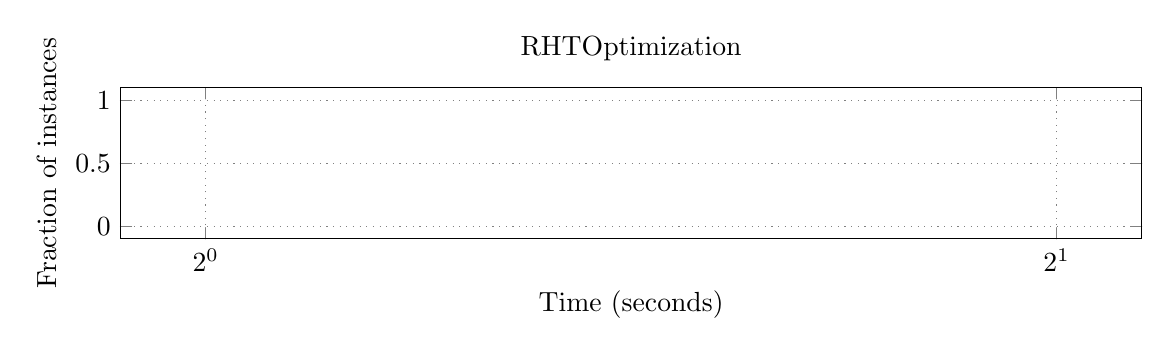
\begin{tikzpicture}
  \begin{axis}[
    title={RHTOptimization},
    xlabel={Time (seconds)},
    ylabel={Fraction of instances},
    xmode=log,
    log basis x={2},
    width=1.2\linewidth,
    height=3.5cm,
    grid=major,
    legend style={
        at={(0.5,-0.2)},
        anchor=north,
    },
    mark=*,
    mark size=0pt,
    line width=0.5pt
    ]
    %% MULTIPLOT \
    %% SELECT x, y, RHTOptimization as color FROM (
    %%   SELECT
    %%     total_time AS x,
    %%     (rn) * 1.0 / total_count AS y,
    %%     RHTOptimization,
    %%     ROW_NUMBER() OVER (PARTITION BY RHTOptimization, bucket ORDER BY total_time) as row_in_bucket
    %%   FROM (
    %%     SELECT
    %%       total_time,
    %%       RANK() OVER (PARTITION BY RHTOptimization ORDER BY total_time) as rn,
    %%       COUNT(*) OVER (PARTITION BY RHTOptimization) as total_count,
    %%       NTILE(500) OVER (PARTITION BY RHTOptimization ORDER BY total_time) AS bucket,
    %%       RHTOptimization
    %%     FROM stats
    %%     WHERE init_num_keys >= 1048576 AND index_name = 'DeLI-Static-Payload'
    %%   )
    %% )
    %% WHERE row_in_bucket = 1
    %% ORDER BY RHTOptimization, x
  \end{axis}
\end{tikzpicture}
\end{subfigure}
\hfill
\begin{subfigure}{0.24\textwidth}
\centering
\begin{tikzpicture}
  \begin{axis}[
    title={SIMDLanes},
    xlabel={Time (seconds)},
    ylabel={Fraction of instances},
    xmode=log,
    log basis x={2},
    width=1.2\linewidth,
    height=3.5cm,
    grid=major,
    legend style={
        at={(0.5,-0.2)},
        anchor=north,
    },
    mark=*,
    mark size=0pt,
    line width=0.5pt
    ]
    %% MULTIPLOT \
    %% SELECT x, y, SIMDLanes as color FROM (
    %%   SELECT
    %%     total_time AS x,
    %%     (rn) * 1.0 / total_count AS y,
    %%     SIMDLanes,
    %%     ROW_NUMBER() OVER (PARTITION BY SIMDLanes, bucket ORDER BY total_time) as row_in_bucket
    %%   FROM (
    %%     SELECT
    %%       total_time,
    %%       RANK() OVER (PARTITION BY SIMDLanes ORDER BY total_time) as rn,
    %%       COUNT(*) OVER (PARTITION BY SIMDLanes) as total_count,
    %%       NTILE(500) OVER (PARTITION BY SIMDLanes ORDER BY total_time) AS bucket,
    %%       SIMDLanes
    %%     FROM stats
    %%     WHERE init_num_keys >= 1048576 AND index_name = 'DeLI-Static-Payload'
    %%   )
    %% )
    %% WHERE row_in_bucket = 1
    %% ORDER BY SIMDLanes, x
  \end{axis}
\end{tikzpicture}
\end{subfigure}
\hfill
\begin{subfigure}{0.24\textwidth}
\centering
\begin{tikzpicture}
  \begin{axis}[
    title={RHTLoad},
    xlabel={Time (seconds)},
    ylabel={Fraction of instances},
    xmode=log,
    log basis x={2},
    width=1.2\linewidth,
    height=3.5cm,
    grid=major,
    legend style={
        at={(0.5,-0.2)},
        anchor=north,
    },
    mark=*,
    mark size=0pt,
    line width=0.5pt
    ]
    %% MULTIPLOT \
    %% SELECT x, y, RHTLoad as color FROM (
    %%   SELECT
    %%     total_time AS x,
    %%     (rn) * 1.0 / total_count AS y,
    %%     RHTLoad,
    %%     ROW_NUMBER() OVER (PARTITION BY RHTLoad, bucket ORDER BY total_time) as row_in_bucket
    %%   FROM (
    %%     SELECT
    %%       total_time,
    %%       RANK() OVER (PARTITION BY RHTLoad ORDER BY total_time) as rn,
    %%       COUNT(*) OVER (PARTITION BY RHTLoad) as total_count,
    %%       NTILE(500) OVER (PARTITION BY RHTLoad ORDER BY total_time) AS bucket,
    %%       RHTLoad
    %%     FROM stats
    %%     WHERE init_num_keys >= 1048576 AND index_name = 'DeLI-Static-Payload'
    %%   )
    %% )
    %% WHERE row_in_bucket = 1
    %% ORDER BY RHTLoad, x
  \end{axis}
\end{tikzpicture}
\end{subfigure}
\hfill
\begin{subfigure}{0.24\textwidth}
\centering
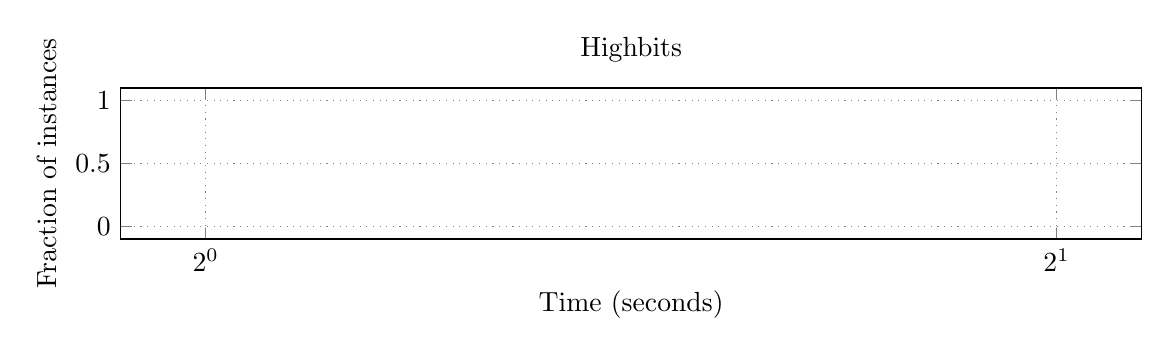
\begin{tikzpicture}
  \begin{axis}[
    title={Highbits},
    xlabel={Time (seconds)},
    ylabel={Fraction of instances},
    xmode=log,
    log basis x={2},
    width=1.2\linewidth,
    height=3.5cm,
    grid=major,
    legend style={
        at={(0.5,-0.2)},
        anchor=north,
    },
    mark=*,
    mark size=0pt,
    line width=0.5pt
    ]
    %% MULTIPLOT \
    %% SELECT x, y, Highbits as color FROM (
    %%   SELECT
    %%     total_time AS x,
    %%     (rn) * 1.0 / total_count AS y,
    %%     Highbits,
    %%     ROW_NUMBER() OVER (PARTITION BY Highbits, bucket ORDER BY total_time) as row_in_bucket
    %%   FROM (
    %%     SELECT
    %%       total_time,
    %%       RANK() OVER (PARTITION BY Highbits ORDER BY total_time) as rn,
    %%       COUNT(*) OVER (PARTITION BY Highbits) as total_count,
    %%       NTILE(500) OVER (PARTITION BY Highbits ORDER BY total_time) AS bucket,
    %%       Highbits
    %%     FROM stats
    %%     WHERE init_num_keys >= 1048576 AND index_name = 'DeLI-Static-Payload'
    %%   )
    %% )
    %% WHERE row_in_bucket = 1
    %% ORDER BY Highbits, x
  \end{axis}
\end{tikzpicture}
\end{subfigure}
\hfill
\caption{Performance plots for DeLI-Static-Payload index on all workloads and distributions (init key size $2^{i}, i \in [20 , 25]$).}
\end{figure}



\section{DeLI Dynamic Payload}\label{sec:delidynamicpayload}

\subsection{Performance plot (all workloads and distributions)}

\begin{figure}[H]
\small
\centering

\begin{subfigure}{0.24\textwidth}
\centering
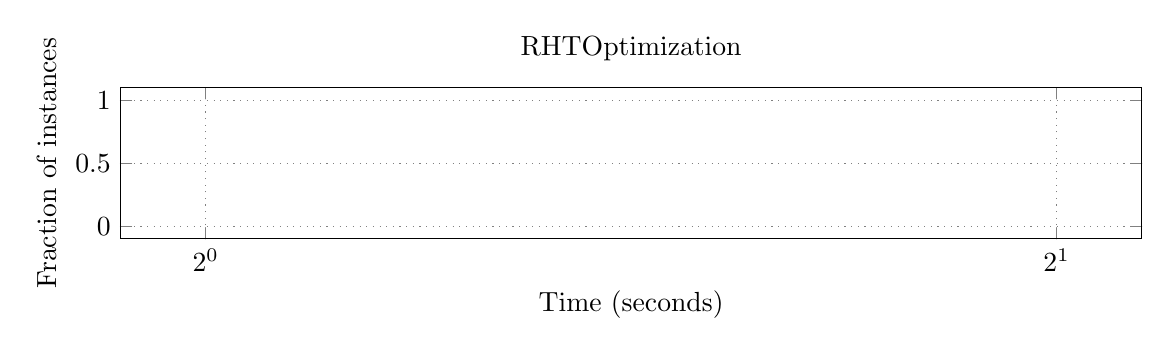
\begin{tikzpicture}
  \begin{axis}[
    title={RHTOptimization},
    xlabel={Time (seconds)},
    ylabel={Fraction of instances},
    xmode=log,
    log basis x={2},
    width=1.2\linewidth,
    height=3.5cm,
    grid=major,
    legend style={
        at={(0.5,-0.2)},
        anchor=north,
    },
    mark=*,
    mark size=0pt,
    line width=0.5pt
    ]
    %% MULTIPLOT \
    %% SELECT x, y, RHTOptimization as color FROM (
    %%   SELECT
    %%     total_time AS x,
    %%     (rn) * 1.0 / total_count AS y,
    %%     RHTOptimization,
    %%     ROW_NUMBER() OVER (PARTITION BY RHTOptimization, bucket ORDER BY total_time) as row_in_bucket
    %%   FROM (
    %%     SELECT
    %%       total_time,
    %%       RANK() OVER (PARTITION BY RHTOptimization ORDER BY total_time) as rn,
    %%       COUNT(*) OVER (PARTITION BY RHTOptimization) as total_count,
    %%       NTILE(500) OVER (PARTITION BY RHTOptimization ORDER BY total_time) AS bucket,
    %%       RHTOptimization
    %%     FROM stats
    %%     WHERE init_num_keys >= 1048576 AND index_name = 'DeLI-Dynamic-Payload'
    %%   )
    %% )
    %% WHERE row_in_bucket = 1
    %% ORDER BY RHTOptimization, x
  \end{axis}
\end{tikzpicture}
\end{subfigure}
\hfill
\begin{subfigure}{0.24\textwidth}
\centering
\begin{tikzpicture}
  \begin{axis}[
    title={SIMDLanes},
    xlabel={Time (seconds)},
    ylabel={Fraction of instances},
    xmode=log,
    log basis x={2},
    width=1.2\linewidth,
    height=3.5cm,
    grid=major,
    legend style={
        at={(0.5,-0.2)},
        anchor=north,
    },
    mark=*,
    mark size=0pt,
    line width=0.5pt
    ]
    %% MULTIPLOT \
    %% SELECT x, y, SIMDLanes as color FROM (
    %%   SELECT
    %%     total_time AS x,
    %%     (rn) * 1.0 / total_count AS y,
    %%     SIMDLanes,
    %%     ROW_NUMBER() OVER (PARTITION BY SIMDLanes, bucket ORDER BY total_time) as row_in_bucket
    %%   FROM (
    %%     SELECT
    %%       total_time,
    %%       RANK() OVER (PARTITION BY SIMDLanes ORDER BY total_time) as rn,
    %%       COUNT(*) OVER (PARTITION BY SIMDLanes) as total_count,
    %%       NTILE(500) OVER (PARTITION BY SIMDLanes ORDER BY total_time) AS bucket,
    %%       SIMDLanes
    %%     FROM stats
    %%     WHERE init_num_keys >= 1048576 AND index_name = 'DeLI-Dynamic-Payload'
    %%   )
    %% )
    %% WHERE row_in_bucket = 1
    %% ORDER BY SIMDLanes, x
  \end{axis}
\end{tikzpicture}
\end{subfigure}
\hfill
\begin{subfigure}{0.24\textwidth}
\centering
\begin{tikzpicture}
  \begin{axis}[
    title={RHTLoad},
    xlabel={Time (seconds)},
    ylabel={Fraction of instances},
    xmode=log,
    log basis x={2},
    width=1.2\linewidth,
    height=3.5cm,
    grid=major,
    legend style={
        at={(0.5,-0.2)},
        anchor=north,
    },
    mark=*,
    mark size=0pt,
    line width=0.5pt
    ]
    %% MULTIPLOT \
    %% SELECT x, y, RHTLoad as color FROM (
    %%   SELECT
    %%     total_time AS x,
    %%     (rn) * 1.0 / total_count AS y,
    %%     RHTLoad,
    %%     ROW_NUMBER() OVER (PARTITION BY RHTLoad, bucket ORDER BY total_time) as row_in_bucket
    %%   FROM (
    %%     SELECT
    %%       total_time,
    %%       RANK() OVER (PARTITION BY RHTLoad ORDER BY total_time) as rn,
    %%       COUNT(*) OVER (PARTITION BY RHTLoad) as total_count,
    %%       NTILE(500) OVER (PARTITION BY RHTLoad ORDER BY total_time) AS bucket,
    %%       RHTLoad
    %%     FROM stats
    %%     WHERE init_num_keys >= 1048576 AND index_name = 'DeLI-Dynamic-Payload'
    %%   )
    %% )
    %% WHERE row_in_bucket = 1
    %% ORDER BY RHTLoad, x
  \end{axis}
\end{tikzpicture}
\end{subfigure}
\hfill
\begin{subfigure}{0.24\textwidth}
\centering
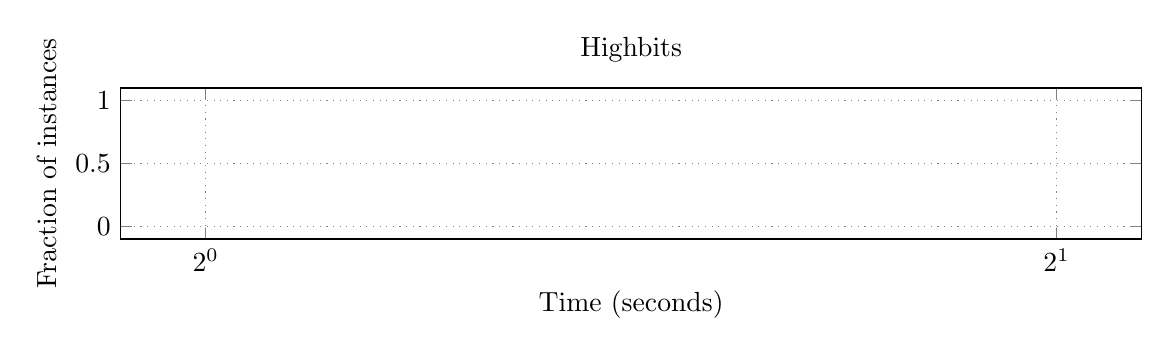
\begin{tikzpicture}
  \begin{axis}[
    title={Highbits},
    xlabel={Time (seconds)},
    ylabel={Fraction of instances},
    xmode=log,
    log basis x={2},
    width=1.2\linewidth,
    height=3.5cm,
    grid=major,
    legend style={
        at={(0.5,-0.2)},
        anchor=north,
    },
    mark=*,
    mark size=0pt,
    line width=0.5pt
    ]
    %% MULTIPLOT \
    %% SELECT x, y, Highbits as color FROM (
    %%   SELECT
    %%     total_time AS x,
    %%     (rn) * 1.0 / total_count AS y,
    %%     Highbits,
    %%     ROW_NUMBER() OVER (PARTITION BY Highbits, bucket ORDER BY total_time) as row_in_bucket
    %%   FROM (
    %%     SELECT
    %%       total_time,
    %%       RANK() OVER (PARTITION BY Highbits ORDER BY total_time) as rn,
    %%       COUNT(*) OVER (PARTITION BY Highbits) as total_count,
    %%       NTILE(500) OVER (PARTITION BY Highbits ORDER BY total_time) AS bucket,
    %%       Highbits
    %%     FROM stats
    %%     WHERE init_num_keys >= 1048576 AND index_name = 'DeLI-Dynamic-Payload'
    %%   )
    %% )
    %% WHERE row_in_bucket = 1
    %% ORDER BY Highbits, x
  \end{axis}
\end{tikzpicture}
\end{subfigure}
\hfill
\caption{Performance plots for DeLI-Dynamic-Payload index on all workloads and distributions (init key size $2^{i}, i \in [20 , 25]$).}
\end{figure}

\section{Best Variants Performance}\label{sec:best}

\subsection{Performance plot (best variant per index)}

\begin{figure}[H]
\small
\centering
\begin{tikzpicture}
  \begin{axis}[
    title={Best variants},
    xlabel={Time (seconds)},
    ylabel={Fraction of instances},
    xmode=log,
    log basis x={2},
    width=150mm,
    height=100mm,
    grid=major,
    legend pos=south east,
    mark=*,
    mark size=0pt,
    line width=0.5pt
    ]
    %% MULTIPLOT \
    %% SELECT x, y, index_name as color FROM (
    %%   SELECT
    %%     total_time AS x,
    %%     (rn) * 1.0 / total_count AS y,
    %%     index_name,
    %%     ROW_NUMBER() OVER (PARTITION BY index_name, bucket ORDER BY total_time) as row_in_bucket
    %%   FROM (
    %%     SELECT
    %%       total_time,
    %%       RANK() OVER (PARTITION BY index_name ORDER BY total_time) as rn,
    %%       COUNT(*) OVER (PARTITION BY index_name) as total_count,
    %%       NTILE(1000) OVER (PARTITION BY index_name ORDER BY total_time) AS bucket,
    %%       index_name
    %%     FROM stats_best
    %%     WHERE init_num_keys >= 1048576
    %%   )
    %% )
    %% WHERE row_in_bucket = 1
    %% ORDER BY index_name, x
  \end{axis}
\end{tikzpicture}
\caption{Performance plots for best index variants (init key size $2^{i}, i \in [20 , 25]$).}
\end{figure}

\end{document}
